\section{Introduction}
In recent years, improvements in embedded processing technology have allowed for the creation of robotic situational awareness platforms for remotely observing dangerous or inaccessible areas. The market for such devices is a new and expanding field, and faces large demand from the military and first responders. This field is being piloted by throwable and remotely drivable platforms such as the Endeavor Robotics 110 FirstLook and the Bounce Imaging Explorer, shown in Figure \ref{robocop}. 

\par
\begin{figure}[H]
        \begin{subfigure}[h]{0.5\textwidth}
             \centerline{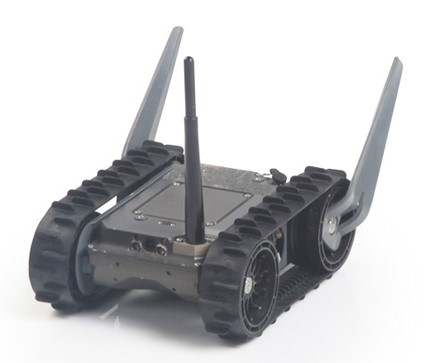
\includegraphics[width=1.0\textwidth]{FirstLook.jpg}}
            \caption{Endeavor Robotics 110 FirstLook \cite{endeavor}}
        \end{subfigure}
        \begin{subfigure}[h]{0.5\textwidth}
            \centerline{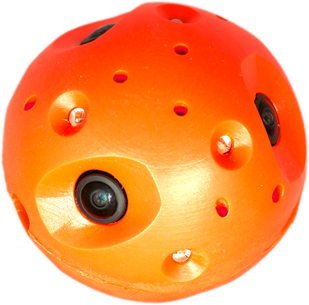
\includegraphics[width=0.8\textwidth]{bounce_img.png}}
            \caption{Bounce Imaging Explorer \cite{bounceImaging}}
        \end{subfigure}
\caption{Robotic Situational Awareness Devices}
\label{robocop}
\end{figure}
\par
These devices contain simple wireless video streaming technology, allowing for remote visual surveillance. Although a video stream is an effective strategy for simple observation, this method of gathering information has room for improvement. This project investigated the extraction of information such as object positioning and localization from a camera-based sensor suite in real time, allowing for more comprehensive situational observation. One method of performing this process is through the use of Simultaneous Localization and Mapping, or SLAM. 
\par
SLAM is a technique of mapping an unknown environment with respect to an agent, and can be performed using a wide variety of sensors and computational methods. This technique is a common area of research in the fields of image processing and high-speed computing, and has been applied mainly to autonomous vehicles. Most current SLAM implementations rely on the use of a sensor suite connected to a computer or System on Chip (SoC) computing device. 
\par
One type of technology useful for performing the high speed data processing necessary for an embedded SLAM device is a Field Programmable Gate Array, or FPGA. FPGAs consist of digital circuitry that is designed to be user-configured, allowing for the creation of completely customized digital hardware. FPGAs are especially useful for parallelized data processing, posing potential real-time advantages over standard computing or microcontroller technology. Although FPGA technology is highly applicable to performing SLAM-like tasks, there are currently few existing products that use FPGAs for this purpose. 
\par
This project explored the viability of an FPGA-based real-time SLAM sensor suite as a replacement for standard video cameras on existing situational awareness systems. This sensor suite utilized data from stereo camera modules, a scanning laser rangefinder, and an Inertial Measurement Unit (IMU) to create a real-time depth-augmented video feed and a 2D floorplan from the device's field of view.
\par
The following chapters detail the creation of this sensor suite, beginning with an exploration of relevant technology and prior work. Next, the overall system design of the project is included with a system block diagram. Then, each individual sensor’s implementation is explored in more detail. Methods for processing and combining sensor data to produce the intended 2D floorplan and 3D map visualizations are included. Comprehensive test results are then examined in detail for all sensors and main algorithms used. Lastly, conclusions and recommendations for future improvements are presented. 
